\chapter{Hardware Trust}
Lets first define what trust is.
\begin{boxH}
  A trusted component, operation, or process is one whose \textbf{behavior} is \textbf{predictable}
  under almost \textbf{any} operating \textbf{condition} and which is highly resistant to subversion
  by application software, virus, and a given level or physical interference.
\end{boxH}
The main focus is on the predictable behaviour, for example the root of trust needs to always behave
in the expected manner because its misbehaviour cannot be detected.\\
Trust in the Roots of Trust can be achieved through a variety of means, and it is used as a basic
block for a \textbf{chain of trust}.

\begin{section}{Trust Anchor}
  \begin{boxH}
    A Hardware Trust Anchor is a component that securely store and provide a unique secure
    identifier for the device.
  \end{boxH}
  Since attack difficulty is at the highest with the hardware, it presents an excellent anchor for
  the compute security features.

\end{section}

\begin{section}{Hardware Root-of-Trust Properties}
  The root of trust should:
  \begin{itemize}
    \item be proof of authenticity and/or provenance 
    \item be immutable hardware component(s)
    \item be an anchor trust against a specific threat model
  \end{itemize}

  \begin{figure}[H]
    \centering
    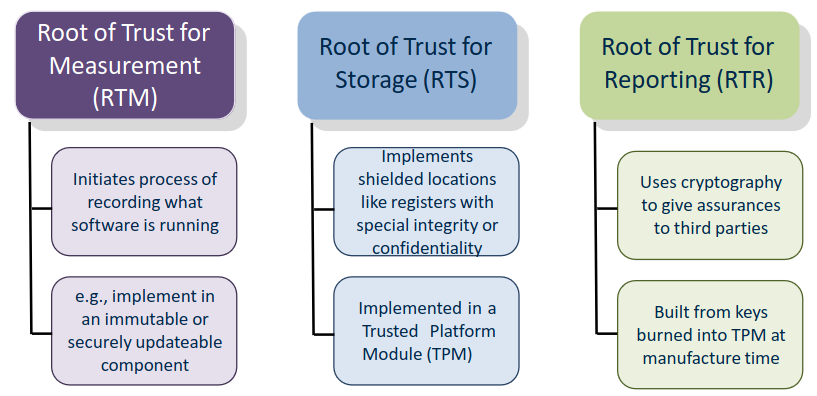
\includegraphics[width=0.7\textwidth]{img/hardware/rot schema.png}
    \caption{Roots of Trust in Trusted Computing}
  \end{figure}
\end{section}

\begin{section}{Trusted Platform Module}
  \begin{boxH}
    A \textbf{Trusted Platform Module} (TPM) is a tamper-resistant integrated circuit built into
    some computer motherboards that can perform \textbf{cryptographic operations} (including key
    generation) and protect small amounts of sensitive information, such as passwords and
    cryptographic keys.
  \end{boxH}

  The specification were initially released in 2003, with the actual version being 2.0.\\
  There are five types of TPM:
  \begin{itemize}
    \item Discrete
    \item Integrated
    \item Firmware
    \item Software
    \item Virtual/Hypervisor
  \end{itemize}
  \textbf{Discrete} TPM is the most common and the \textbf{most secure} form.
  \begin{figure}[H]
    \centering
    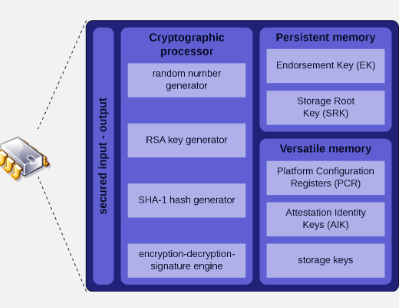
\includegraphics[width=0.5\textwidth]{img/hardware/tcb schema.png}
    \caption{General TPM Architecture}
  \end{figure}
  \begin{subsection}{Trusted Computing Base}
    \begin{boxH}
      With Trusted Computing Base we refer to the totality of protection mechanisms within a
      computer system, including hardware, firmware, and software, the combination responsible for
      enforcing a security policy.
    \end{boxH}
    TPM has become standard in many consumer-grade computers over the last few years, in fact every
    secure computing system must have some \textbf{Trusted Computing base}, rooted in hardware, small
    and isolated from the rest of the computing components, which correctness and state should be
    easily and independently verifiable.\\
    The TPM provides hardware-based authentication, integrity, and attestation to the TCB, and
    provides the following functions:
    \begin{itemize}
      \item A root-of-trust for reporting and storage
      \item Measurement and attestation of platform integrity
      \item Platform identification and authentication
      \item Core and highly constrained cryptographic functions
    \end{itemize}
  \end{subsection}
  The TPM provides many basic features, like:
  \begin{itemize}
    \item Secure Boot & Firmware Integrity
    \item Certification
    \item Attestation and Authentication
    \item Protected Location
    \item Integrity Measurements and Reporting
  \end{itemize}
  \begin{subsection}{Secure Boot \& Firmware Integrity}
    The environment in which the code runs must be controlled, in fact a power-on reset creates an
    environment in which the platform is in a well- known initial state.\\
    \begin{boxH}
      Secure Boot is the act of establishing a \textbf{secure initial state}.
    \end{boxH}
    The typical secure boot method verifies the authenticity of each component in the boot chain.
    With secure boot we have \textit{two bootloaders}: the first one is stored in a secure memory
    and verifies the integrity and authenticity of the second one, while the second one verifies the 
    integrity and authenticity of the OS kernel and of the firmware. This implies that the first
    bootloader cannot be modified.
    \begin{figure}[H]
      \centering
      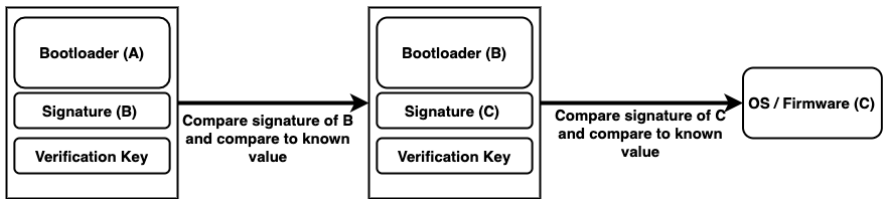
\includegraphics[width=0.7\textwidth]{img/hardware/secure boot.png}
      \caption{Secure Boot}
    \end{figure}
  \end{subsection}

  \begin{subsection}{Certification}
    A certificate of authenticity should be available for the key shipped with the TPM:
    \begin{itemize}
      \item It can be used to associate credentials (certificate) with other TPMs
      \item A certified key that can be used for signing may be used to attest the platform data
        that affect the integrity (trustworthiness) of a platform
    \end{itemize}
    Certificate and authentication credential can be stored in a Root of Trust for Storage (RTS)
    element.
  \end{subsection}

  \begin{subsection}{Attestation and Authentication}
    Root of Trust components are usually the entities trusted when attesting to a
    devices
    \begin{itemize}
      \item Unique identifiers can be stored in a Root of Trust element and used to identify the
        system
      \item A unique identifier can be obtained by resorting to Physically Unclonable Functions
        (PUFs)
    \end{itemize}
    These various attestation takes the form of keys, certificates, software signature, etc. that
    are stored inside the TPM.

  \end{subsection}
  \begin{subsection}{Protected Location}
    All information on a TPM is in a \textbf{Shielded Location}, which content is not disclosed
    unless intended: only the allowed entities can access the secure memory and the Root of Trust
    functionalities.\\
    When sensitive data are not stored in a Shielded Location on the TPM, they are encrypted and are
    said to be in a \textbf{Protected Location}. Encryption of Protected Locations uses multiple
    seeds and keys that never leave the TPM, and tamper resistent devices are used to avoid
    disclosing sensitive information to common physical attacks.
  \end{subsection}

  \begin{subsection}{Integrity Measurments and Reporting}
    An integrity measurement is a value that represents a possible change in the trust state of the
    platform.\\
    The measured object may be:
    \begin{itemize}
      \item A data value
      \item The hash of code or data
    \end{itemize}
    The digest of an arbitrary set of integrity measurements is statistically unique.
  \end{subsection}
\end{section}

\begin{section}{Trusted Execution Environments}
  With the current situation, trusted/untrusted code run on trusted/untrusted cores, but this
  situation is not ideal.\\
  During the years a new trust-aware architectural framework have been developed, to integrate
  multiple heterogeneous IPs or tenants, secure to non-secure cores, in the same chip design.
  This allows to virtualize the hardware trough trusted, untrusted and unknows core islands.

  \begin{figure}[H]
    \centering
    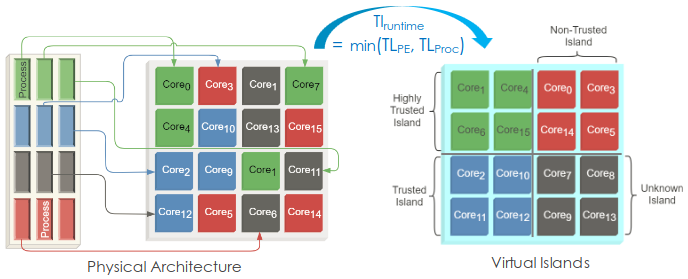
\includegraphics[width=0.7\textwidth]{img/hardware/virtual islands.png}
    \caption{The virtual islands partitioning}
  \end{figure}

  \begin{boxH}
    \textbf{Trusted Execution Environments} (TEEs) are secure systems-on-chip areas guaranteeing
    code and data protection.
  \end{boxH}
  They typically offer the minimal security required by low-end, closed embedded systems, such as
  IoT and “bare-metal” (i.e., without any Operating System) solutions.\\
  TEE was originally an initiative of Global Platform to standardize a part of the processor as a
  trusted, secure part but has since evolved and covers, in general, the hardware modifications made
  to processors to provide isolation and attestation to software.

\end{section}

\begin{section}{Memory Protection Unit}
  Each memory page can be read, written, or executed just by a predefined set of tasks/processes.
  Access rights are decided by the kernel, which runs privileged
  The MPU automatically processes addresses sent to the memory without the intervention of the
  kernel, and violations cause the immediate abortion of the task.
  \begin{figure}[H]
    \centering
    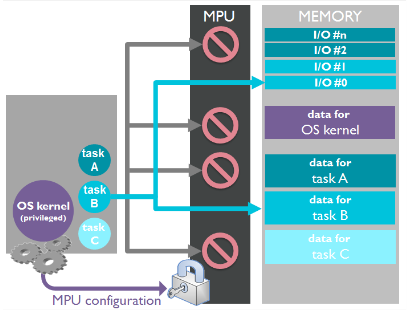
\includegraphics[width=0.4\textwidth]{img/hardware/memory protection unit.png}
    \caption{Memory Protection Unit}
  \end{figure}

\end{section}

\begin{section}{Device level solutions}
  A set of solutions was adopted at the device level to improve the device’s resistance and
  resiliency to external attacks.
  \begin{subsection}{Tamper-evident devices}
    \begin{boxH}
      Tamper-evident devices are devices that include some indicator of compromise, automatically
      activated when someone tries to mess with its physical integrity.
    \end{boxH}
    At the physical level, packaging should maximize the evidence of tampering, and additional
    internal sensors (e.g., light detectors, temperature sensors, \dots) could be inserted to detect
    the presence of laser rays used to perform fault injection attacks.\\
    At the software level, appropriate auditing mechanisms through logging procedures to trace
    conducted activities and their sources should be implemented.
  \end{subsection}

  \begin{subsection}{Tamper-resistant devices}
    \begin{boxH}
      Tamper-resistant devices are devices that are properly engineered in a way to reduce the
      surface for physical attacks.
    \end{boxH}
    The main idea is the strengthening of the hardware physical shielding, for example chips that
    are destroyed by any attempt of decapsulation, or ones with stronger packaging.
  \end{subsection}
\end{section}

\begin{section}{Security Oriented Components}
  Those are components with a set of custom, special purpose components used for performing specific
  security-oriented operations, including:
  \begin{itemize}
    \item Hardware Cyphers
    \item Smart Cards \& SIM Cards
    \item Secure storage devices
    \item Random Number Generators
  \end{itemize}

  \begin{subsection}{Hardware Cyphers}
    \begin{boxH}
      Hardware Cyphers are custom devices used to assist or replace software in cryptographic
      operations.
    \end{boxH}
    Hardware implementation are:
    \begin{itemize}
      \item faster
      \item less prone to exploitation than software
    \end{itemize}
    Furthermore, they can be isolated from the main processor, with only a small subset of entities
    can access their functionalities. This means that even if the main system is compromised, the
    integrity of hardware ciphers can be guaranteed.
  \end{subsection}

  \begin{subsection}{Smart Cards and Sim}
    Smart cards are device that are able to provide a different range of security solutions, like
    authentication mechanism based on ownership, but they are basically a CPU linked to an I/O
    system.\\
    They can provide:
    \begin{itemize}
      \item A set of hardware-accelerated cryptographic algorithms
      \item Public keys and secret keys
      \item Secure key generation and storage
    \end{itemize}
    A sim in a type of smart card.
  \end{subsection}

  \begin{subsection}{Secure Storage Devices}
    Securing stored data is a prime concern in many applications
    A secure storage device must be designed and manufactured in a way that defines a certain level
    of protection:
    \begin{itemize}
      \item Tamper-evident devices
      \item Tamper-resistant devices
      \item Secure authentication mechanism
      \item Drive’s controller security
      \item Data encryption
      \item Secure Erase
    \end{itemize}
    \begin{subsection}{Secure Authentication Mechanism}
      Hacking the authentication mechanism is far easier than breaking the underlying encryption
      mechanism.\\
      Four possible authentication mechanisms are:
      \begin{itemize}
        \item \textbf{PIN pad}: can be subjected to a very simple exploit. Some buttons may present
          signs of usage, hence revealing the input combination
        \item \textbf{Software PIN input}: in this case, PIN must never be stored in software to
          mitigate replay attacks of eventual software vulnerabilities
        \item \textbf{Wireless badge}: they can be easily cloned
        \item \textbf{Fingerprint}: if the input system is not properly manufactured, it can be
          bypassed even without the need to fake the owner's fingerprint
      \end{itemize}
    \end{subsection}

    \begin{subsection}{Drive’s Controller Security}
      The drive’s controller must be developed to prevent unwanted access to the device
      The drive’s controller must present some protection against brute force attacks:
      \begin{itemize}
        \item Blocking after a series of unsuccessful authentication
        \item Deleting encryption keys and information stored in flash
        \item Avoid that passwords, PINs, or encryption keys can be requested to the drive’s
          controller (trivial, but it happens)
      \end{itemize}
    \end{subsection}

    \begin{subsection}{Secure Erase}
      Storage need for proper data sanitization techniques, even in case of disposal. An erase
      operation usually consists of overwriting all data with a given value, either 0 or 1.\\
      In solid state drive, data are stored as an electric charge, and even a simple overwrite
      operation may leave some residual charge that, by using appropriate measurement equipment, can
      be measured to retrieve old data. This means that multiple write operations are needed to
      completely remove any correlation between residual charges and old stored data.

    \end{subsection}

  \end{section}
